\chapter{Introduction}\label{chapter:intro}

\section{Code testing}

\blindtext

\begin{minted}{haskell}
quicksort [] = []
quicksort (p:xs) = (quicksort lesser) ++ [p] ++ (quicksort greater)
    where
    lesser = filter (< p) xs
    greater = filter (>= p) xs
\end{minted}

This is a sample text for footnote \footnote{First footnote \blindtext} and
some following text.

\section{math testing}

\[
\begin{bmatrix}
    a  &  b \\
    c  &  d      
\end{bmatrix}
= 
\begin{bmatrix}
    8  &  1 \\
    7  &  6      
\end{bmatrix}
\]

\section{Citation testing}

Some quote from \emph{A Song of Ice and Fire}\cite{dance-with-dragons}

\section{Table testing}

\begin{table}[htb]
    \centering
    \begin{tabular}{lccc}
        & Not Presented & Presented & Used \\
        Diet Article       & 118           & 266       & 101  \\
        Dinosaur Article   & 121           & 273       & 136  \\
        Government Article & 105           & 277       & 148 
    \end{tabular}
    \caption{Number of participants for each experimental article}
\end{table}

\section{Image testing}

In figure \ref{fig:dos} we something.

\begin{figure}[!h]
    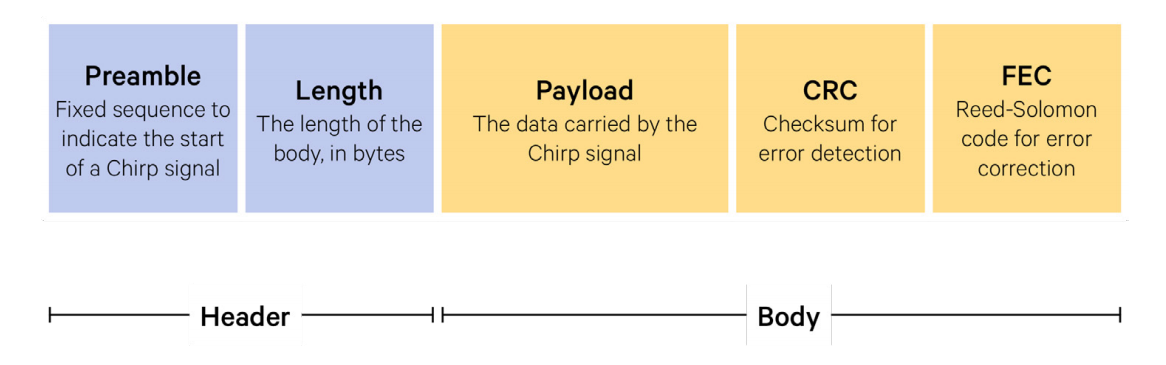
\includegraphics[width=\linewidth]{res/dos_message.png}
    \caption{Data over sound}
    \label{fig:dos}
\end{figure}
